\subsection{Conditioned-Target Object Detector}
\label{sec:cond_target_obj_detector}
In this section, we will present the architecture designed for the \textit{scene analysis task}. Specifically, starting with the current agent observation $o_{t}$ and the command representation $d_{task}$, our objective is to explicitly locate the target object within the agent scene by predicting its bounding-box $bb_{t}$. In the realm of Computer Vision, Object Detection is a well-established and extensively researched problem, with modern methods achieving high levels of performance in detection and classification tasks. However, we cannot directly apply these methods, as made in \cite{jiang2023vima, zhu2023viola}, because our goal is not to identify all objects in the scene or a specific category of objects. Instead, we aim to identify the \textit{\textbf{target object}}, which can vary depending on the task at hand, while maintaining the methods class-agnostic nature (i.e., it does not predict the object category).
\newline To address this task, we drew inspiration from the `Visual Question and Answering' problem \ref{sec:research_activity}. Our approach is rooted in the concept that, much like the architecture presented in \cite{perez2018film} can direct attention to specific regions of an image in response to input queries, we aim for our model to exhibit a similar ability. Specifically, we want the model to focus on a particular portion of the image based on the task command $d_{task}$.
The proposed architecture is reported in Figure \ref{fig:ctod}
\begin{figure}[htb]
    \centering
    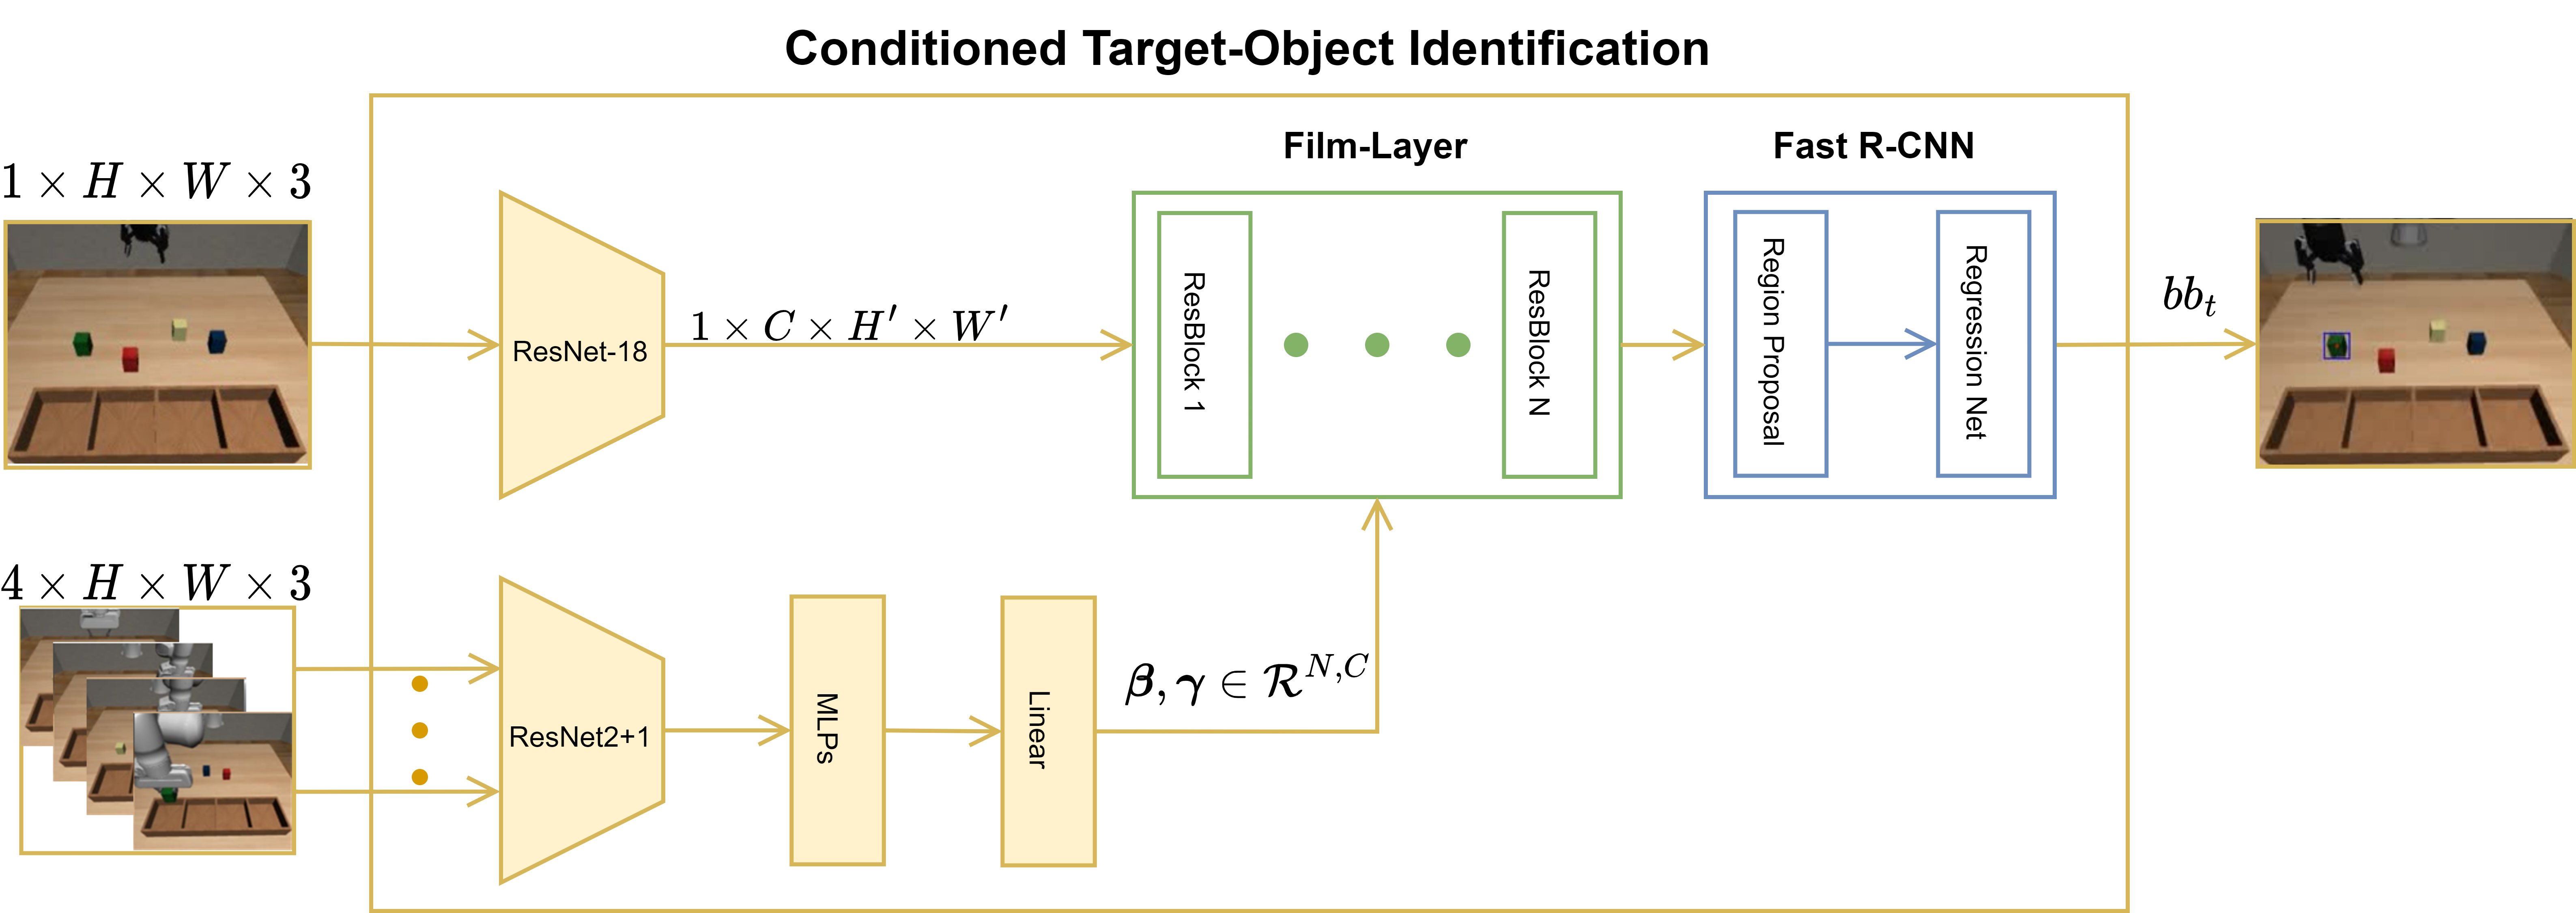
\includegraphics[width=0.8\textwidth]{Figures/images/ctod/ctod.png}
    \caption{Proposed architecture for solving the Conditioned-Target Object Detector}
    \label{fig:ctod}
\end{figure}

It is composed by the following modules:
\begin{itemize}
    \item \textit{ResNet-18} \cite{resnet}, as feature-extractor for the agent observazione $o_{t}$, rapresented as an RGB image.
    \item \textit{ResNet2+1} \cite{resnet21},  as a feature extractor for the command description $d_{t}$. This description is represented by a set of 4 frames sampled from the demonstrator's execution video. The chosen architecture facilitates the extraction of both spatial and temporal features. Subsequently, the generated features are flattened and processed through a Multilayer Perceptron (MLP) network.
    \item The FiLM-Layer, as introduced in \cite{perez2018film}, serves as the module responsible for integrating the features derived from both the agent and command processing stages. In detail, this layer carries out a modulation of the $c^{th}$ activation through a feature-wise affine transformation, expressed as $FiLM(\textbf{F}{c}|\gamma{c}, \beta_{c}) = \gamma_{c} \textbf{F}{c} + \beta{c}$. Here, $\gamma$ and $\beta$ represent parameters generated by the linear module, based on the desired input.
    \item \textit{Fast R-CNN} \cite{fastrcnn}, is the dual-stage anchor-based object-detector.
\end{itemize}
The whole architecture has been trained according to the classic object-detector loss-function $\mathcal{L} = w_{1}\mathcal{L}_{reg} + w_{2}\mathcal{L}_{cls} + w_{3}\mathcal{L}_{class}$, where: \begin{itemize}
    \item $\mathcal{L}_{reg}$ is the \textit{L1-loss} function that compares the predicted bounding-box offset and the ground truth offset.
    \item $\mathcal{L}_{cls}$ is a \textit{binary-cross entropy loss} that allows the model to learn the difference between foreground and background bounding-box.
    \item $\mathcal{L}_{class}$ is a cross-entropy loss designed to accommodate object classification. In our scenario, owing to the class-agnostic nature of our model, we trained it to distinguish between two object classes: \textit{target} and \textit{no-target}.
\end{itemize}
\begin{table}[htb]
    \centering
    \fontsize{11pt}{11pt}
    \selectfont
    \caption{Conditioned-Target Object Detector performance}
    \label{table:ctod_performance}
    \resizebox{\linewidth}{!}{%
        \begin{tabular}{>{\centering\hspace{0pt}}m{0.304\linewidth}>{\centering\hspace{0pt}}m{0.335\linewidth}>{\centering\arraybackslash\hspace{0pt}}m{0.263\linewidth}}
            \hline
            \textbf{Task} & \textbf{Precision@0.5} & \textbf{Recall@0.5} \\
            \hline
            Pick-Place    & 0.87                   & 0.99                \\
            \hline
            Nut-Assembly  & 0.96                   & 0.99                \\
            \hline
        \end{tabular}
    }
\end{table}
The model's performance is documented in Table \ref{table:ctod_performance}, and it is evident that we have achieved a highly stable detector in terms of both precision and recall. This stability is maintained throughout various phases, encompassing the initial frames when the robot approaches the target object and during the manipulation itself. For a quantitative analysis of prediction distribution in both pick-place and nut-assembly scenarios, please refer to Table \ref{table:ctdo_prediction_distribution}. It's worth noting the remarkably low number of false-negative predictions, indicating instances where the target object was not detected. In contrast, the false-positive cases are limited to just \textbf{192} predictions in pick-place and \textbf{52} cases in nut-assembly, characterized by predicted bounding boxes with an Intersection Over Union (IoU) of zero. Figure \ref{fig:ctdo_trajectory_execution} presents a specific example of predictions during a trajectory execution. Despite an IoU of less than 0.5, the prediction remains in close proximity to the target object. These results underscore the potential of the proposed system in providing valuable information to address the initial step in the Decision-Making process, which is detailed in Section \ref{sec:research_topic}.
\begin{table}[bth!]
    \centering
    \caption{Conditioned Target Object Detector prediction distribution}
    \fontsize{10pt}{10pt}
    \selectfont
    \label{table:ctdo_prediction_distribution}
    \begin{tblr}{
        width = \linewidth,
        colspec = {Q[185]Q[73]Q[162]Q[177]Q[162]Q[177]},
        cells = {c},
        hlines,
        hline{1,4} = {-}{0.08em},
            }
        {\textbf{Task } \\\textbf{(\#Frames)}} & \textbf{TP} & {\textbf{FP }\\\textbf{pre-picking}} & {\textbf{FP }\\\textbf{post-picking}} & {\textbf{FN }\\\textbf{pre-picking}} & {\textbf{FN }\\\textbf{post-picking}} \\
        {Pick-Place     \\(11229)}                & 9718        & 625                                  & 812                                   & 74                                   & 0                                     \\
        {Nut-Assembly   \\(5643)}                & 5187        & 186                                  & 80                                    & 10                                   & 0
    \end{tblr}
\end{table}
\begin{figure}[bth!]
    \centering
    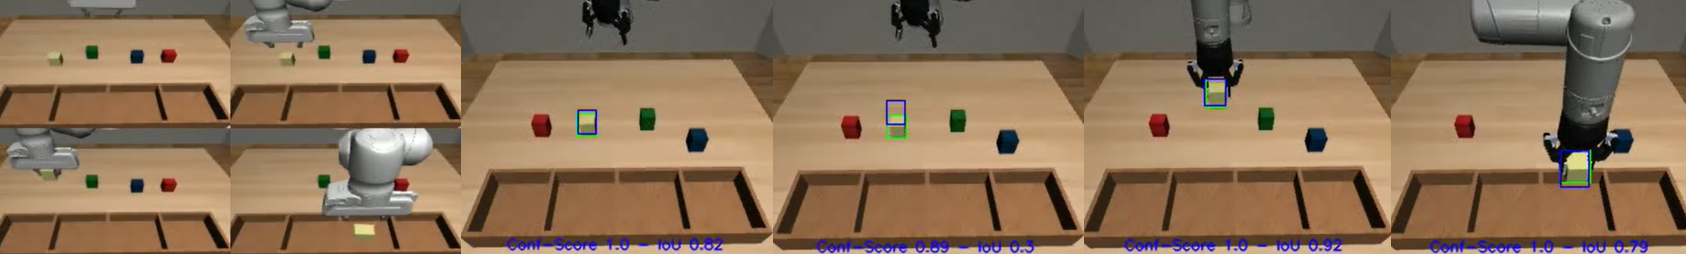
\includegraphics[width=0.9\textwidth]{Figures/images/object_detector/example_prediction.png}
    \caption{Example of predictions during trajectory execution}
    \label{fig:ctdo_trajectory_execution}
\end{figure}

